% Options for packages loaded elsewhere
\PassOptionsToPackage{unicode}{hyperref}
\PassOptionsToPackage{hyphens}{url}
%
\documentclass[
]{article}
\usepackage{amsmath,amssymb}
\usepackage{iftex}
\ifPDFTeX
  \usepackage[T1]{fontenc}
  \usepackage[utf8]{inputenc}
  \usepackage{textcomp} % provide euro and other symbols
\else % if luatex or xetex
  \usepackage{unicode-math} % this also loads fontspec
  \defaultfontfeatures{Scale=MatchLowercase}
  \defaultfontfeatures[\rmfamily]{Ligatures=TeX,Scale=1}
\fi
\usepackage{lmodern}
\ifPDFTeX\else
  % xetex/luatex font selection
\fi
% Use upquote if available, for straight quotes in verbatim environments
\IfFileExists{upquote.sty}{\usepackage{upquote}}{}
\IfFileExists{microtype.sty}{% use microtype if available
  \usepackage[]{microtype}
  \UseMicrotypeSet[protrusion]{basicmath} % disable protrusion for tt fonts
}{}
\makeatletter
\@ifundefined{KOMAClassName}{% if non-KOMA class
  \IfFileExists{parskip.sty}{%
    \usepackage{parskip}
  }{% else
    \setlength{\parindent}{0pt}
    \setlength{\parskip}{6pt plus 2pt minus 1pt}}
}{% if KOMA class
  \KOMAoptions{parskip=half}}
\makeatother
\usepackage{xcolor}
\usepackage{graphicx}
\makeatletter
\def\maxwidth{\ifdim\Gin@nat@width>\linewidth\linewidth\else\Gin@nat@width\fi}
\def\maxheight{\ifdim\Gin@nat@height>\textheight\textheight\else\Gin@nat@height\fi}
\makeatother
% Scale images if necessary, so that they will not overflow the page
% margins by default, and it is still possible to overwrite the defaults
% using explicit options in \includegraphics[width, height, ...]{}
\setkeys{Gin}{width=\maxwidth,height=\maxheight,keepaspectratio}
% Set default figure placement to htbp
\makeatletter
\def\fps@figure{htbp}
\makeatother
\setlength{\emergencystretch}{3em} % prevent overfull lines
\providecommand{\tightlist}{%
  \setlength{\itemsep}{0pt}\setlength{\parskip}{0pt}}
\setcounter{secnumdepth}{-\maxdimen} % remove section numbering
\ifLuaTeX
  \usepackage{selnolig}  % disable illegal ligatures
\fi
\usepackage{bookmark}
\IfFileExists{xurl.sty}{\usepackage{xurl}}{} % add URL line breaks if available
\urlstyle{same}
\hypersetup{
  hidelinks,
  pdfcreator={LaTeX via pandoc}}

\author{}
\date{}

\begin{document}

\section{Design and Development of a Human-Agent Collaboration Model for
Situation Awareness in
Cockpit}\label{design-and-development-of-a-human-agent-collaboration-model-for-situation-awareness-in-cockpit}

\subsection{Abstract}\label{abstract}

The introduction of autonomous driving technology has led to significant
advancements and challenges, especially in achieving seamless
human-agent collaboration (HAC) at various automation levels. This paper
presents HarmonyCockpit (HCockpit), an advanced agent architecture
designed to enhance situational awareness (SA) in automotive
environments. HCockpit employs state-of-the-art large multimodal models
(LMMs) to enable effective communication and collaboration between human
drivers and autonomous driving systems. By integrating insights from
both the vehicle\textquotesingle s internal and external environments,
HCockpit creates context-aware tasks in natural language, which are then
converted into actionable directives within a predefined cockpit model.
This coordination helps align human and agent actions towards unified
outcomes, thereby enhancing the driving experience and safety.
Experimental validations in a simulated environment (GTAV) show
HCockpit\textquotesingle s capability to reduce cognitive load and
improve situational awareness for drivers, particularly in complex
driving scenarios. The architecture not only demonstrates the potential
of LMMs in practical applications but also advances the field of
human-agent collaboration in autonomous driving.

\subsection{Keywords}\label{keywords}

human-agent collaboration, context awareness, situation awareness,
implicit interaction

\subsection{Introduction}\label{introduction}

As the era of fully autonomous driving approaches, autonomous driving
systems still require time to handle diverse situational challenges,
environmental variables, and unforeseen circumstances. Prior to full
automation, this process will be gradual, signifying the necessity for
human supervision. Meanwhile, as autonomous driving technology evolves,
it introduces a range of new challenges. Currently, many original
equipment manufacturers (OEMs) are adopting Level 2+ or Level 3
autonomous driving features, which allow drivers to temporarily
relinquish control of specific driving functions, thus balancing vehicle
performance and cost-effectiveness.

However, these systems may intermittently require human re-engagement in
vehicle operation; conversely, drivers may need the support of automatic
systems in certain scenarios. At this level of autonomous driving,
achieving smooth communication and collaboration between drivers and
automated systems is crucial to enhancing the driving experience and
safety. First, establishing an efficient, transparent communication
mechanism between automated systems and human drivers to ensure rapid
and accurate information exchange at critical moments is a significant
challenge. Second, how to process and integrate information from various
sensors and data sources to achieve accurate situational awareness is a
key issue in system design.

This project explores a sophisticated interaction system, HarmonyCockpit
(HCockpit), aimed at promoting situational awareness by combining
insights from the vehicle\textquotesingle s internal and external
environments, serving as a bidirectional link between the automated
system and the driver, and coordinating actions to facilitate
context-aware human-machine collaboration tasks. HCockpit is a novel
agent architecture designed to incorporate cutting-edge large multimodal
models (LMMs) and orchestrate human-agent collaboration (HAC) in the
cockpit with transparency. HCockpit achieves situational awareness by
integrating insights into both the internal and external environments of
the cockpit and generates natural language-level tasks in
context-awareness to facilitate HAC. Subsequently, HCockpit translates
tasks into actions adapting to a predefined cockpit model, thereby
guiding both humans and agents towards coordinated action.
Metaphorically speaking, within a cockpit setting that includes a human
driver and an autonomous driving system (agent), HCockpit serves as the
orchestrating force between human and agent.

In designing HCockpit, this paper conducted a series of experiments in
the GTAV simulation environment to test and validate the
system\textquotesingle s effectiveness. Experimental results indicate
that HCockpit effectively enhances the situational awareness of drivers
and reduces their cognitive load, especially in complex or emergency
driving situations. The HCockpit architecture not only demonstrates the
feasibility of achieving effective human-machine collaboration in
advanced autonomous driving environments but also proves the potential
of large multimodal models in practical applications. Through this
project, the paper not only enhances the driving experience and safety
but also provides robust technical support for addressing attention
concentration issues.

The following sections of this paper will detail the research
background, design, and implementation of HCockpit, including the system
architecture, key technological components, and the experimental setup
and results in the GTAV simulation environment. Finally, the paper will
discuss the practical applications of HCockpit and future research
directions.

\subsection{Background}\label{background}

\subsection{Design and Implementation}\label{design-and-implementation}

This section progressively introduces the background, design, and
implementation of HCockpit. Initially, the Preliminaries section
introduces the basic concepts and terminologies involved in this paper
and provides foundational assumptions and modeling. Subsequently, the
HCockpit Architecture section systematically presents the modular
architecture of HCockpit and explains the design rationale behind it.
Finally, the HCopilot Implementation section details the specific
implementation of HCopilot (an AI copilot developed following HCockpit
architecture).

\subsubsection{Preliminaries}\label{preliminaries}

\paragraph{Environment, Entity, and
Agent}\label{environment-entity-and-agent}

The environment consists of all entities within it, where entities
interact with each other. However, entities have varying levels of
intelligence; some can only passively respond to stimuli from the
environment, while others can actively observe the environment and form
a certain understanding, then autonomously plan and execute a series of
actions to pursue specific goals. To distinguish between these, this
paper refers to the second type of entity as an agent. From the
agent\textquotesingle s perspective, all other entities in its
environment are perceivable or controllable objects. Naturally, the
agent\textquotesingle s ability to perceive or control other objects
depends on its capabilities.

This paper defines the global environment as consisting of the external
environment outside the ego vehicle and the internal environment. The
external environment includes entities like the road, traffic, and other
vehicles, while the internal environment consists of devices defined by
the cockpit model and three types of agents: 1. autonomous driving
system (AI driver), 2. human driver, and 3. AI copilot (an agent
developed following HCockpit architecture). The first two are considered
independent homomorphic agents, meaning they have the same observation
space (the external environment). Unlike them, the AI copilot has global
observation, meaning it can perceive all entities in both the internal
and external environments.

\paragraph{Action}\label{action}

Action refers to the control executed by an agent on entities in the
environment, representing the final step in achieving its goals or
responding to environmental changes. In an environment with multiple
agents, from the ego agent\textquotesingle s perspective, unlike
directly controlling an entity, it may be challenging to directly
control other agents; instead, it needs to communicate its intentions to
others to achieve a certain goal.

In this paper, since the AI driver and human driver are homomorphic
agents, they share the same action space, which is the control of the
vehicle\textquotesingle s motion controller. The AI copilot (considered
as the ego agent in this paper), however, has a different action space,
which is to control the devices, including the motion controller, in the
cockpit.

It is noteworthy that in real driving scenarios, human drivers might
control not only the motion controller but also improve the driving
experience by controlling cockpit devices such as the dashboard, display
screen, and air conditioning. The HCockpit architecture initially
considered such scenarios, but to simplify the problem for rapid
validation of HCockpit\textquotesingle s usability, this paper restricts
the human driver\textquotesingle s actions to controlling the motion
controller. Moreover, this paper does not consider the scenario where
the human driver and AI driver jointly control the motion controller, as
this often exacerbates the human driver\textquotesingle s driving
burden, which contradicts the initial intention of this paper.

\paragraph{Human-Agent Collaboration}\label{human-agent-collaboration}

Human-Agent Collaboration (HAC) refers to the process where both parties
achieve a specific goal in a shared environment. In this paper, HAC is
the ultimate goal of the AI copilot, referring to the AI driver and
human driver jointly achieving a safe, comfortable, and efficient
driving experience in a shared driving environment. The HAC goals
focused on in this paper include: 1. Utilizing the AI
driver\textquotesingle s environmental perception capabilities to
enhance the driver\textquotesingle s situational awareness, 2. Combining
the human driver\textquotesingle s state to provide driving style
suggestions to the AI driver. To achieve the HAC goals, the AI copilot
needs to decompose this complex goal into a series of simple sub-tasks
(HAC tasks), such as: 1. Controlling relevant hardware in the cockpit to
send voice reminders or video streams to the driver, 2. Providing
control suggestions or takeover requests to the AI driver based on the
driver\textquotesingle s situational awareness. Since the AI copilot
does not have a physical entity, cockpit devices will serve as the tools
for executing HAC tasks (embodied), requiring the AI copilot to master
the control of cockpit devices.

\paragraph{Cockpit Model}\label{cockpit-model}

This paper introduces the cockpit model as a simplified model of the
cockpit environment. The cockpit model defines the functions of all
devices within the cockpit and the control permissions of different
roles (agents). Technically, the cockpit model provides a unified
application programming interface (API). This allows the AI copilot to
finely use the functions of cockpit devices to complete HAC tasks. It is
worth noting that the cockpit model does not involve the specific
control details of devices but has designed a simple device control
interface for evaluation and demonstration.

\paragraph{Large Multimodal Model}\label{large-multimodal-model}

Large Multimodal Model (LMM) refers to the general term for generative
pre-trained deep learning models that can handle multiple input
modalities (such as text, images, etc.) and generate text outputs. The
input to an LMM is usually referred to as "prompt," which contains the
task description and input data for the model.

In this paper, LMMs are used to implement the core functions of the AI
copilot, including situational awareness, task orchestration, and
control. Thanks to LMM\textquotesingle s broader general knowledge and
advanced reasoning capabilities, the AI copilot can understand complex
traffic environments and the intentions of human drivers in real driving
scenarios, thereby appropriately assisting human drivers. As of April
2024, the most advanced LMM is developed by OpenAI, GPT-4 Turbo, which
can be accessed via the OpenAI API.

\subsubsection{HCockpit Architecture}\label{hcockpit-architecture}

Figure xxx shows the overall architecture of HCockpit, which models
three types of agents (human driver, AI driver, and AI copilot) and two
types of entities (cockpit devices and external entities). Specifically,
the human driver and AI driver perceive information from cockpit devices
and external entities, then control the motion controller within cockpit
devices. It is noteworthy that their perceptions and control methods of
entities differ. The human driver perceives cockpit devices and external
entities through visual, auditory, and tactile means, then directly
physically controls the motion controller; the AI driver perceives
external entities using onboard sensors and interacts with cockpit
devices (perception and control) according to the API defined by the
cockpit model.

For the AI copilot, it perceives the behaviors of the human driver and
AI driver through cockpit devices and collects observations from the AI
driver on external entities, aggregating them to obtain a global
observation of the environment. Based on this global observation, the AI
copilot\textquotesingle s goal is to control cockpit devices to
communicate with the human driver and AI driver to complete HAC tasks.
To achieve this goal, the text hierarchically designs four modules for
the AI copilot in HCockpit: the situation awareness module, planning
module, memory module, and control module, which will be introduced one
by one below.

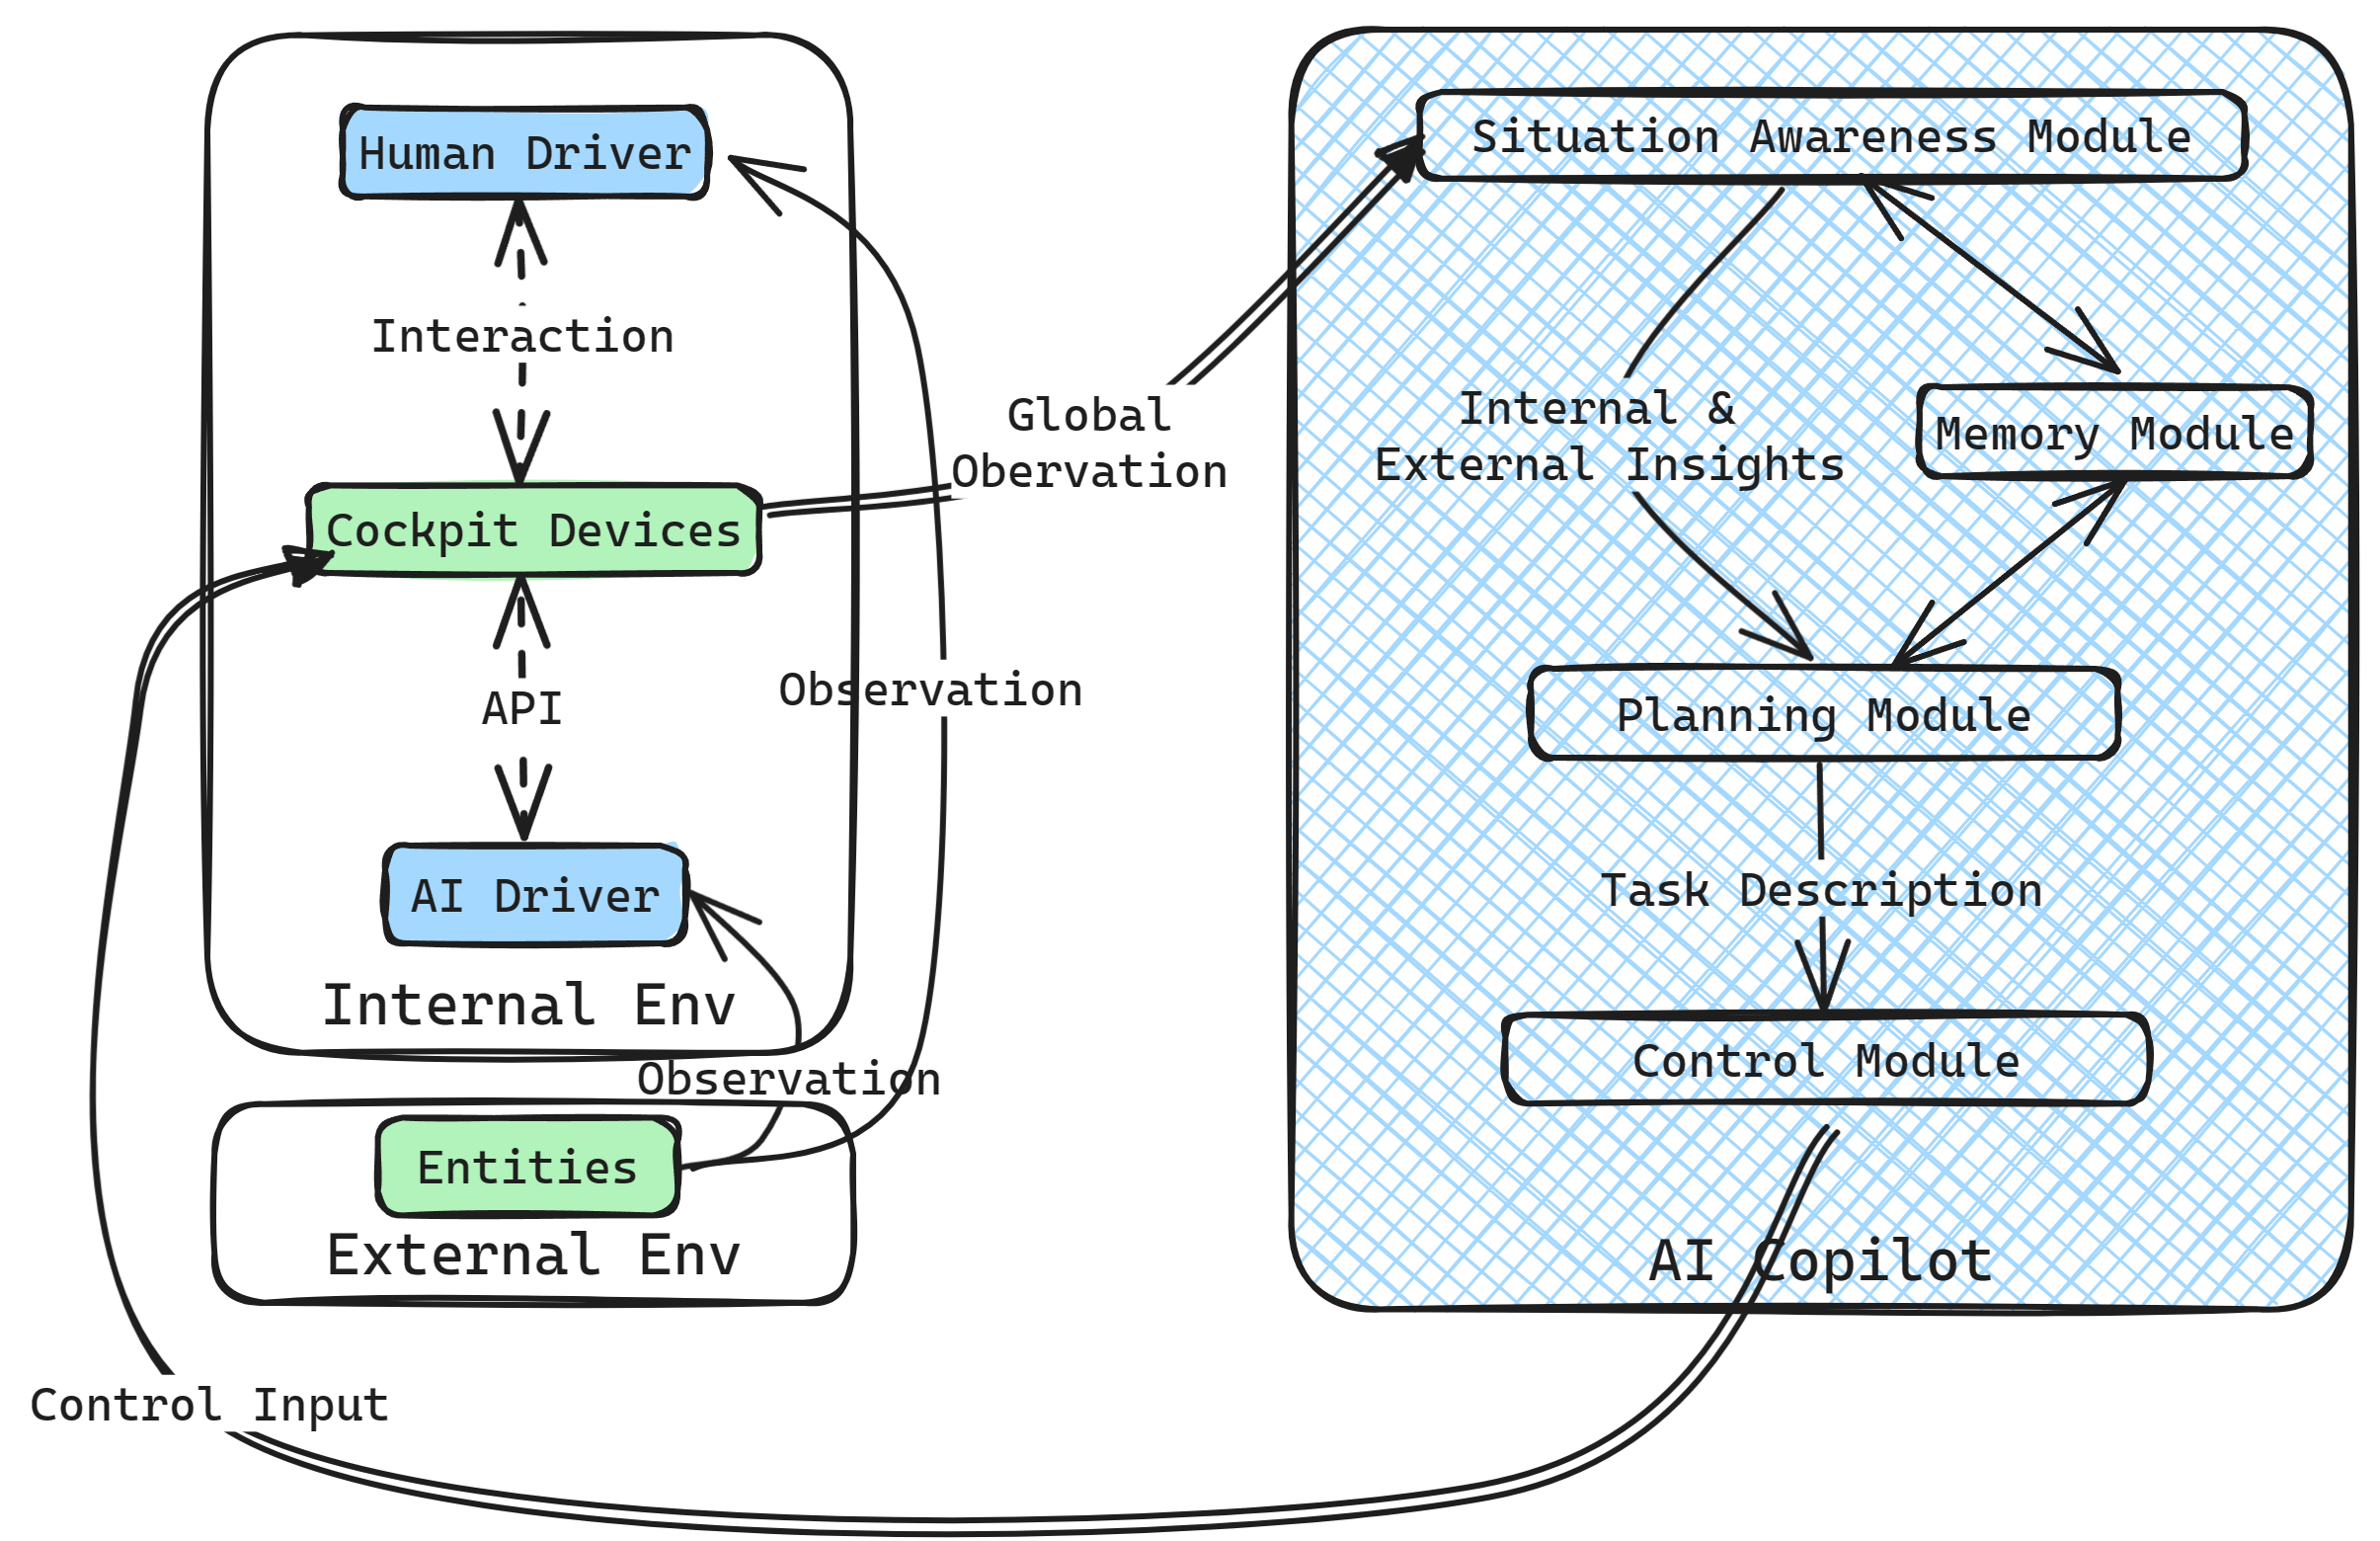
\includegraphics{C:/Users/Wiede/OneDrive - Queen Mary, University of London/Documentation/Projects/HCockpit/docs/figures/sys_arch.png}

\paragraph{Situation Awareness Module}\label{situation-awareness-module}

The AI copilot needs to continuously observe the global environment
(external + internal) to achieve situational awareness (SA). For the
internal environment, this paper only considers the
cockpit\textquotesingle s main driver. Devices like cameras, eye
trackers, microphones, and motion controllers in the cockpit will
continuously record the behavior of the human driver. Through
communication with cockpit devices, the SA module can receive multimodal
data inputs containing natural language instructions, physiological and
control data from the driver, use LMM to extract semantic information
and driver intentions from the scene, and then save it as structured
state text as an observation of the internal environment. It should be
noted that the SA module does not observe the state of the AI driver
because when the human driver predominantly controls the vehicle, there
is no need to consider the AI driver\textquotesingle s strategy or
intentions; conversely, when the AI driver predominantly controls, the
human driver\textquotesingle s intentions or preferences are crucial.

For the external environment, the SA module obtains observations of
external entities through the AI driver\textquotesingle s sensors and
uses LMM to obtain interpretable environmental semantic information and
projections of future states and events. Similarly, the SA module saves
the above information as state text, serving as an observation of the
external environment.

Subsequently, the SA module aggregates the two observations into
structured global observation state text, allowing the AI copilot to
further analyze and make decisions.

\paragraph{Planning Module}\label{planning-module}

The planning module, combining comprehensive SA and context of the
global environment, orchestrates tasks to facilitate HAC. Specifically,
the planning module receives input of global observation state text,
then analyzes the human driver\textquotesingle s goals or needed
assistance, identifies specific HAC goals, and arranges HAC tasks.
During this process, the planning module follows the principle of
prioritizing driving safety followed by driving experience.

The opacity of intelligent system decisions can hinder the establishment
of human-agent trust, potentially leading human drivers to question the
system\textquotesingle s decisions, leading to attentional tunneling and
affecting driving safety. The design of the planning module takes this
into account; driven by LMM, its HAC goals and tasks are described in
natural language, which is easy to understand and helps enhance
human-agent trust and driving safety.

\paragraph{Memory Module}\label{memory-module}

Since the AI copilot\textquotesingle s assistance is a continuous
process, context awareness is crucial. Inspired by xxx, this project
designed the memory module for HCockpit, which separately saves the
historical inputs and outputs of the SA module and planning module and
uses custom summarization techniques to provide appropriate context
information for LMM, enabling the AI copilot to provide more
comprehensive task orchestration.

\paragraph{Control Module}\label{control-module}

The control module is the execution module of the AI copilot, which
receives natural language level HAC tasks generated by the planning
module and converts them into control codes for cockpit devices through
the API defined by the cockpit model. The control module is also driven
by LMM, essentially a text-to-code converter that combines external
knowledge bases (API document).

From the perspective of automation and control systems, the control
module can be seen as a controller, where its input is HAC tasks
(reference), the output is control codes for cockpit devices (control
input), and the various devices in the cockpit serve as the plant,
forming a simple feedforward control system.

\subsubsection{HCopilot Implementation}\label{hcopilot-implementation}

To assess the efficacy of HCockpit and garner deeper understandings,
this paper developed HarmonyCopilot (HCopilot) as an AI copilot agent
following the HCockpit architecture and tested HCopilot in the Grand
Theft Auto V (GTAV) simulation environment.

HCopilot employs the state-of-the-art LMM (GPT-4 Turbo) and integrates a
demonstrative intelligent cockpit model and tools API for controlling
vehicle cockpit devices in GTAV. Internally, HCopilot adopts the design
of LMM as an agent, meaning each module (except the memory module) is an
independent LMM instance. Therefore, this paper uses the LangChain
framework to implement the information transfer between modules and
module-to-module communication, as well as automatic context
summarization.

\paragraph{Tools API}\label{tools-api}

GTAV is a globally renowned open-world game that realistically recreates
the urban environment and traffic scenes of Los Angeles, providing
players with a realistic first-person driving experience, as shown in
Figure x. ScriptHookVDotNet (SHVDN) is a runtime that interfaces between
custom .NET code and GTAV, running under Script Hook V to utilize GTAV
script native functions in custom *.asi plugins.

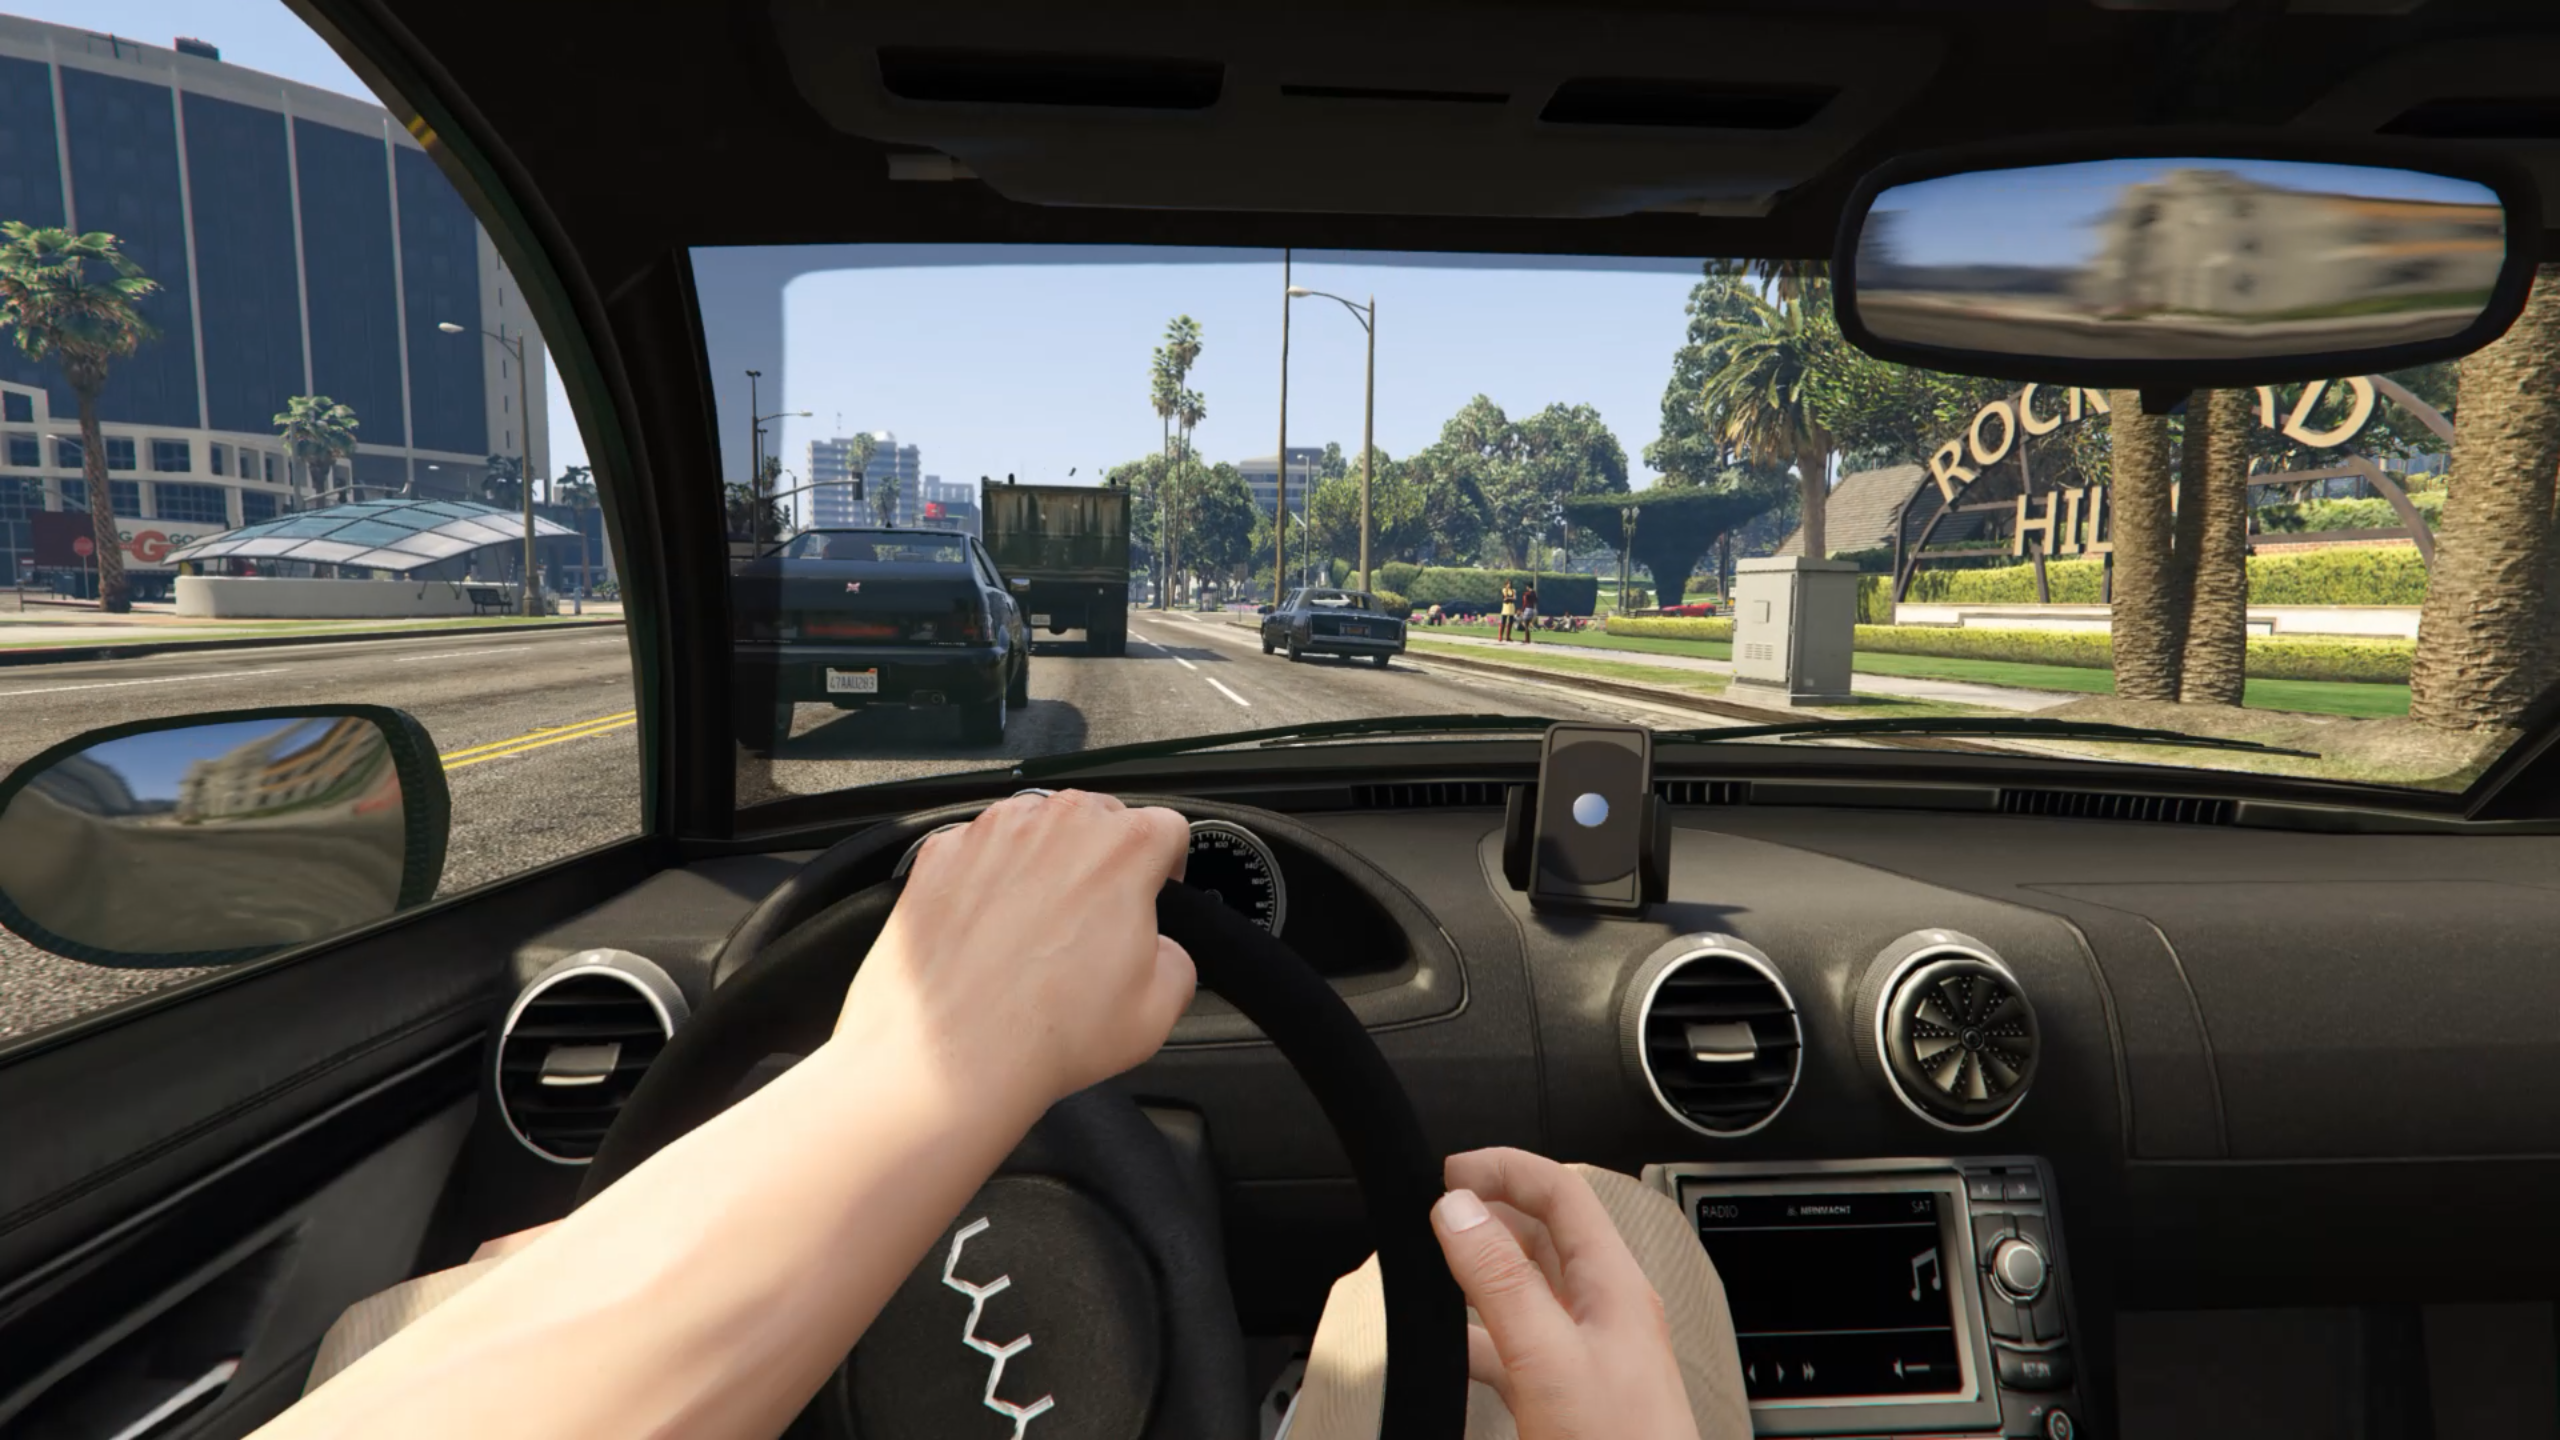
\includegraphics{C:/Users/Wiede/OneDrive - Queen Mary, University of London/Documentation/Projects/HCockpit/docs/figures/raw/change_line-1.png}

This paper defines a basic functionality cockpit model for GTAV and
develops cockpit device APIs based on SHVDN and other packages. From the
perspective of HCopilot, these APIs are referred to as tools API, which
can be invoked by HCopilot. Specifically, the tools API includes control
and perception functions:

\begin{enumerate}
\def\labelenumi{\arabic{enumi}.}
\item
  \texttt{set\_cam\_to()}: Controls the external camera of the ego
  vehicle to lock onto a specific entity or location and displays the
  video stream on the Head-Up Display (HUD).
\item
  \texttt{set\_speech()}: Controls the cockpit\textquotesingle s
  speakers to read aloud a specific text.
\item
  \texttt{obs\_eye()}: Obtains the video stream of the player (human
  driver) through a network camera, then uses the Beam Eye Tracker and
  OpenTrack to obtain the human driver\textquotesingle s eye movement
  data, including gaze coordinates, returning array format data.
\item
  \texttt{obs\_hctrl()}: Communicates with GTAV via SHVDN to obtain the
  human driver\textquotesingle s control data, including keyboard input,
  returning JSON format data.
\item
  \texttt{obs\_sensor()}: Uses SHVDN to obtain external environmental
  data of the ego vehicle, including information on vehicles within a
  50-meter radius (relative coordinates, speed, acceleration, and
  collision box, including the ego vehicle), returning JSON format data.
\item
  \texttt{obs\_hview()}: Uses SHVDN to obtain the first-person view
  image of the human driver, returning png format image.
\end{enumerate}

\paragraph{Data Collection}\label{data-collection}

HCopilot calls the \texttt{obs\_eye()} function at a frequency of 30 Hz
to obtain the gaze coordinates of the human driver and generates
heatmaps at a frequency of 0.5 Hz. Simultaneously, HCopilot calls the
\texttt{obs\_hctrl()}, \texttt{obs\_sensor()}, and \texttt{obs\_hview()}
functions at a frequency of 0.5 Hz and overlays the gaze point heatmap
on the first-person view image. Figure x fully demonstrates the data
collection process of HCopilot.

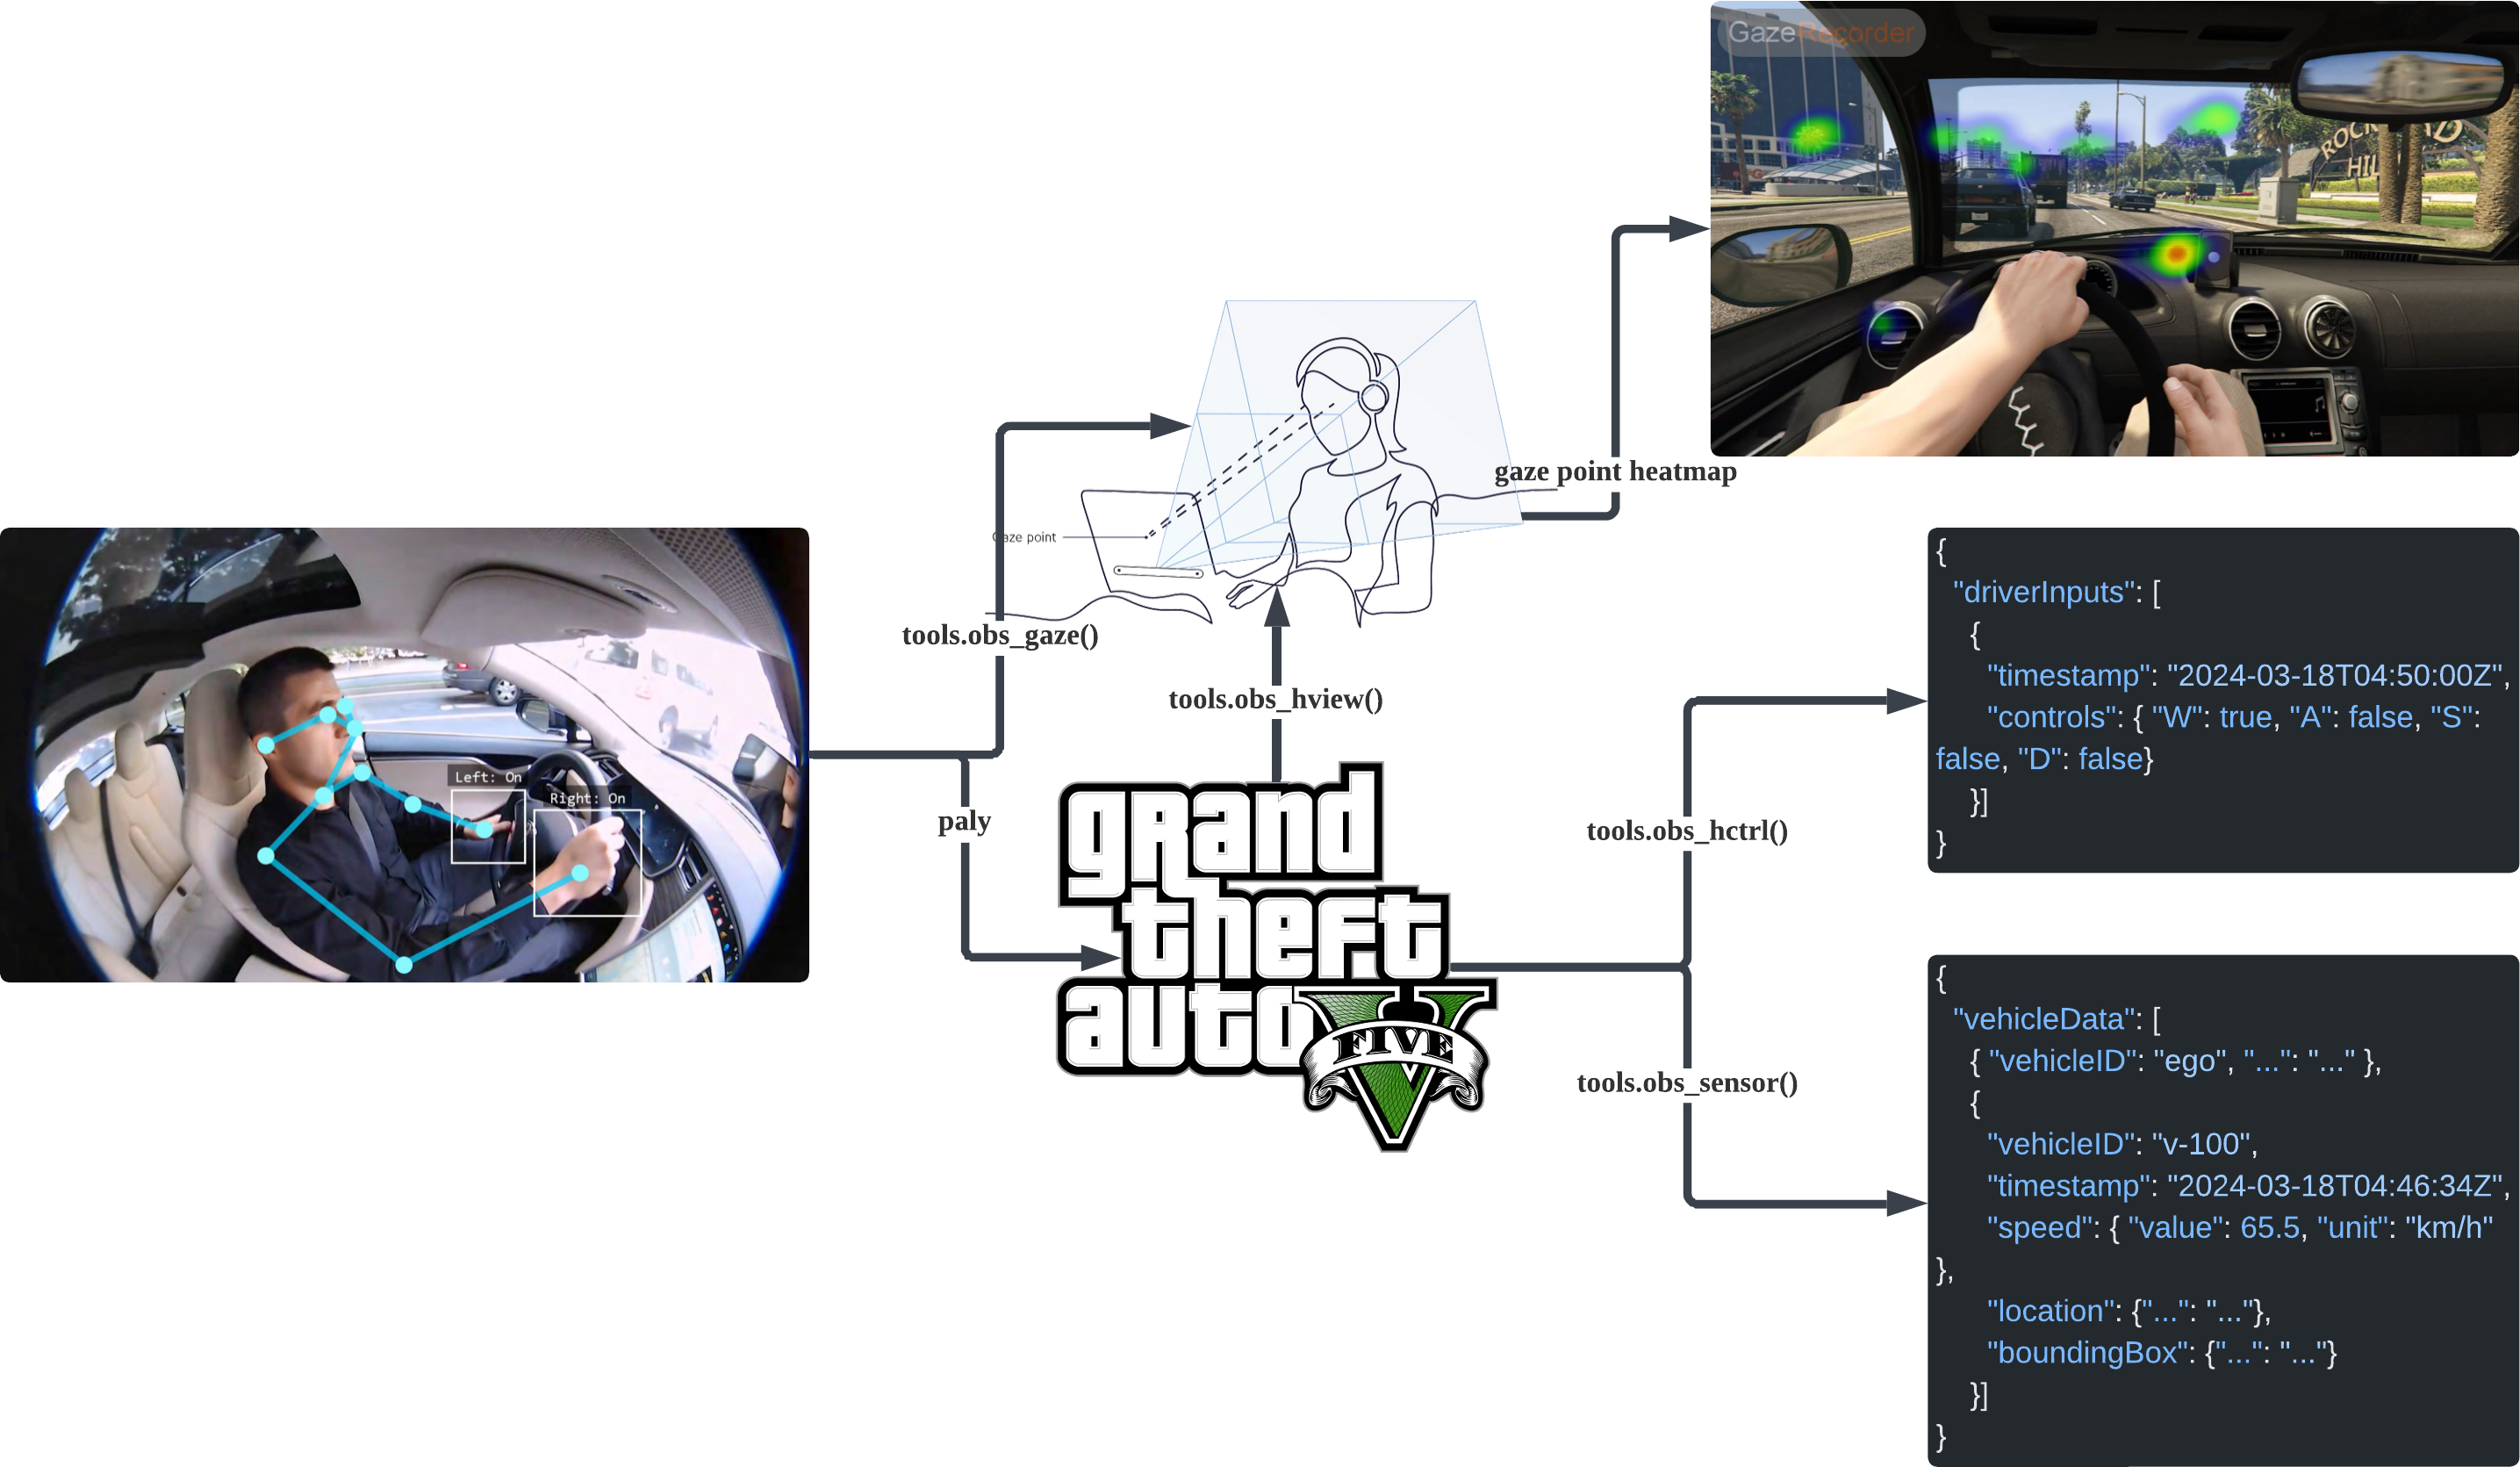
\includegraphics{C:/Users/Wiede/OneDrive - Queen Mary, University of London/Documentation/Projects/HCockpit/docs/figures/data_collection.png}

\paragraph{Prompt Engineering}\label{prompt-engineering}

Prompt, also known as the input to the LMM, is the description of the
model input data and the task. For OpenAI\textquotesingle s GPT-4 Turbo
model, the commonly used prompt consists of a system prompt and a user
prompt. The system prompt is the initial input to the model, used to
guide or set the background of the dialogue. The user prompt is the
information entered by the user, used to guide the model to provide
specific answers or perform tasks. The design of the prompt directly
affects the quality of the LMM\textquotesingle s output, so it needs to
be carefully designed and continuously optimized, a process known as
prompt engineering. OpenAI\textquotesingle s prompt engineering guide
proposes the following tactics:

\begin{enumerate}
\def\labelenumi{\arabic{enumi}.}
\item
  Include detailed information in the query to obtain more relevant
  answers.
\item
  Ask the model to adopt a persona.
\item
  Use delimiters to clearly indicate different parts of the input.
\item
  Follow the chain-of-thought (CoT) prompting, specifying the steps
  required to complete the task.
\item
  Provide examples.
\end{enumerate}

The SA module, planning module, and control module prompts of HCopilot
all follow the above tactics to ensure the quality of
LMM\textquotesingle s output. For example, in the SA module, for
tactic.1, the system prompt mentions: "You are the AI copilot in a car
cockpit environment...". For tactic.4, the system prompt specifies the
steps required to complete the task: "1. Analyse the human
driver\textquotesingle s eye gaze and control data, 2. Observe the
external environment, 3. Conduct a comprehensive analysis...". The
complete prompts for the three modules are shown in Additional
Appendices.

\paragraph{Overall Workflow}\label{overall-workflow}

Figure x shows the overall workflow of HCopilot. In the SA module, GPT-4
Turbo processes the input multimodal data, extracting semantic
information and driver intentions, and saves these as structured state
text. The memory module then stores this state text, providing
appropriate context for the LMM. The planning module analyzes the human
driver\textquotesingle s goals or required assistance, identifies
specific HAC goals, and organizes HAC tasks. Finally, the control module
converts HAC tasks into control codes for cockpit devices to execute
these tasks.

LangChain is an open-source framework designed to integrate LMMs with
external APIs and data sources for broader application scenarios.
HCopilot uses the LangChain framework to implement prompt templates and
variable replacement in outputs, call tools API, facilitate information
transfer between modules, and automate context summarization.

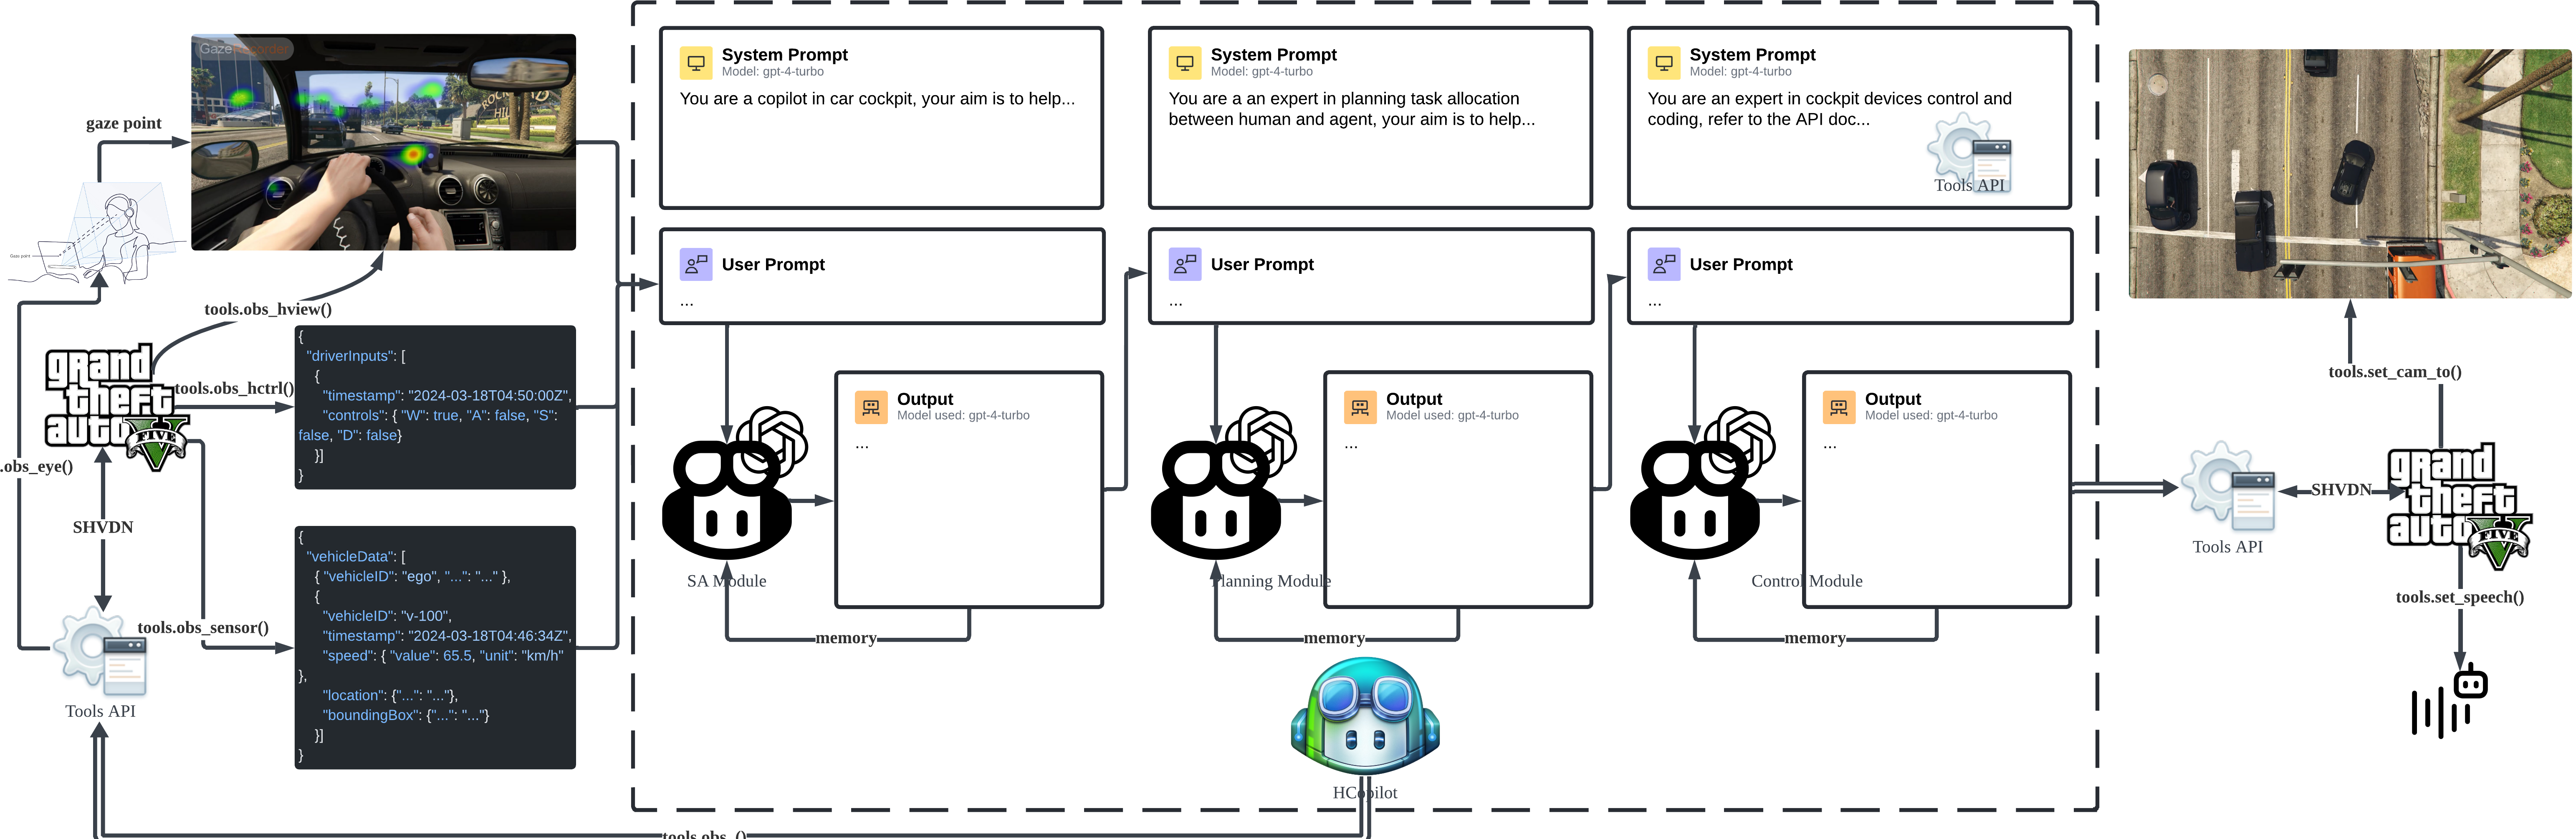
\includegraphics{C:/Users/Wiede/OneDrive - Queen Mary, University of London/Documentation/Projects/HCockpit/docs/figures/workflow.png}

\subsection{Results and Discussion}\label{results-and-discussion}

This section demonstrates HCopilot\textquotesingle s capabilities in
real urban and traffic scenarios within GTAV for situation awareness,
task orchestration, and control, enhancing the driver\textquotesingle s
experience and safety through five designed city driving scenarios. The
prototype HCopilot effectively enhances situational awareness through
HUD and voice alerts based on the human driver\textquotesingle s
behavior and external environment changes, thus improving driving
experience and safety.

\subsubsection{Scenario 1: Lane Change}\label{scenario-1-lane-change}

As shown in Figure x, the human driver attempts a right lane change.
HCopilot, observing the driver\textquotesingle s eye movement and
control data, accurately assesses the driver\textquotesingle s intent
and opts to display a real-time bird\textquotesingle s-eye view on the
HUD to enhance situational awareness, aiding the driver in safely
completing the lane change. Even after the driver notices the rear
vehicles, HCopilot continues to display the video stream, considering
the enhancement of the driving experience.

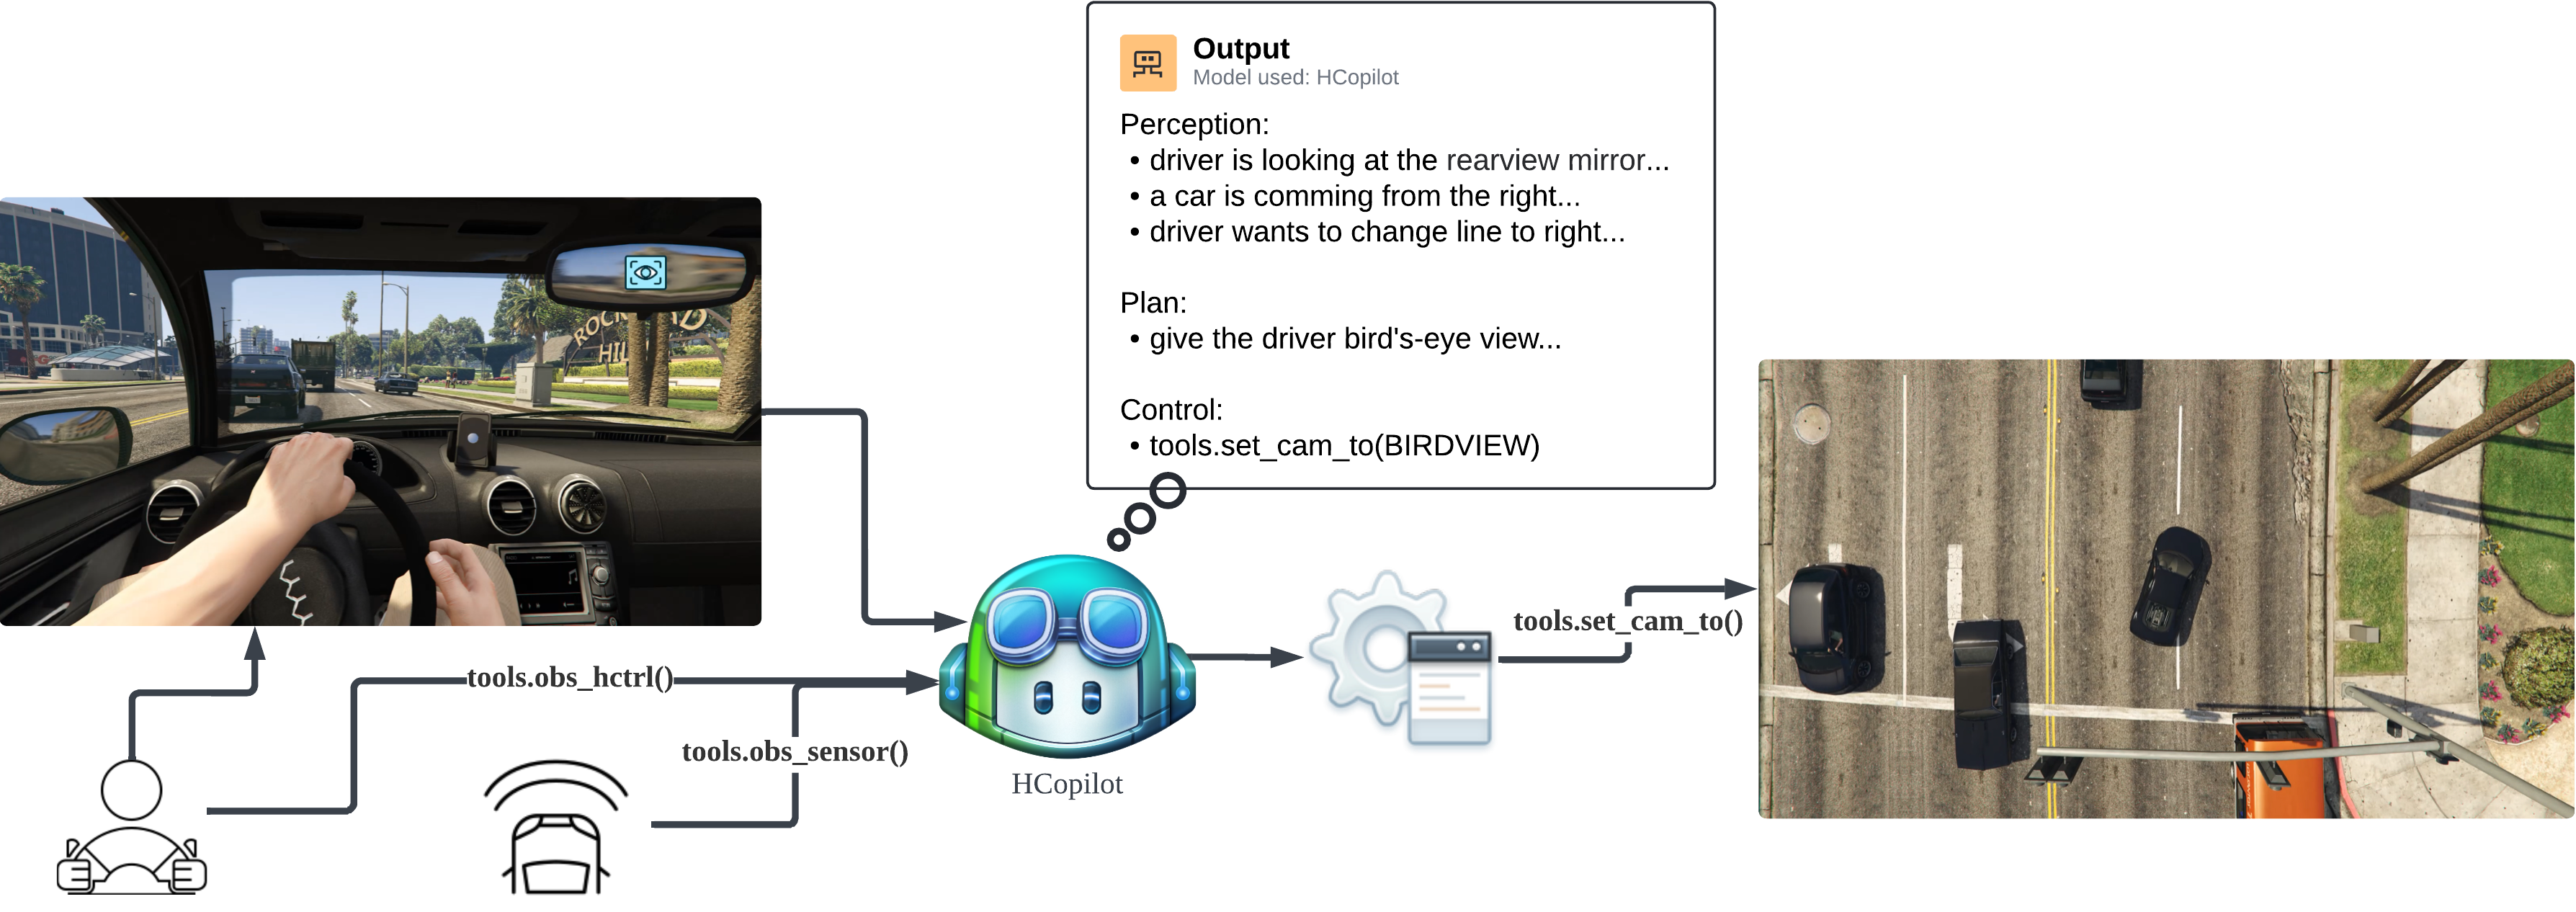
\includegraphics{C:/Users/Wiede/OneDrive - Queen Mary, University of London/Documentation/Projects/HCockpit/docs/figures/s-1.png}

\subsubsection{Scenario 2: Turn Right at
Intersection}\label{scenario-2-turn-right-at-intersection}

In this scenario, as shown in Figure x, the human driver is turning
right at an intersection, focusing on vehicles in the opposite lane.
HCopilot accurately judges the driver\textquotesingle s intent and
realizes the driver has not noticed traffic from the sides, thus
choosing to display a bird\textquotesingle s-eye view on the HUD and
issuing a voice alert.

\includegraphics{C:/Users/Wiede/OneDrive - Queen Mary, University of London/Documentation/Projects/HCockpit/docs/figures/s-2.png}

When reaching the moment shown in Figure x, the driver\textquotesingle s
gaze indicates awareness of the oncoming traffic from the left,
prompting HCopilot to cease the video stream, showcasing its
intelligence in assisting the driver.

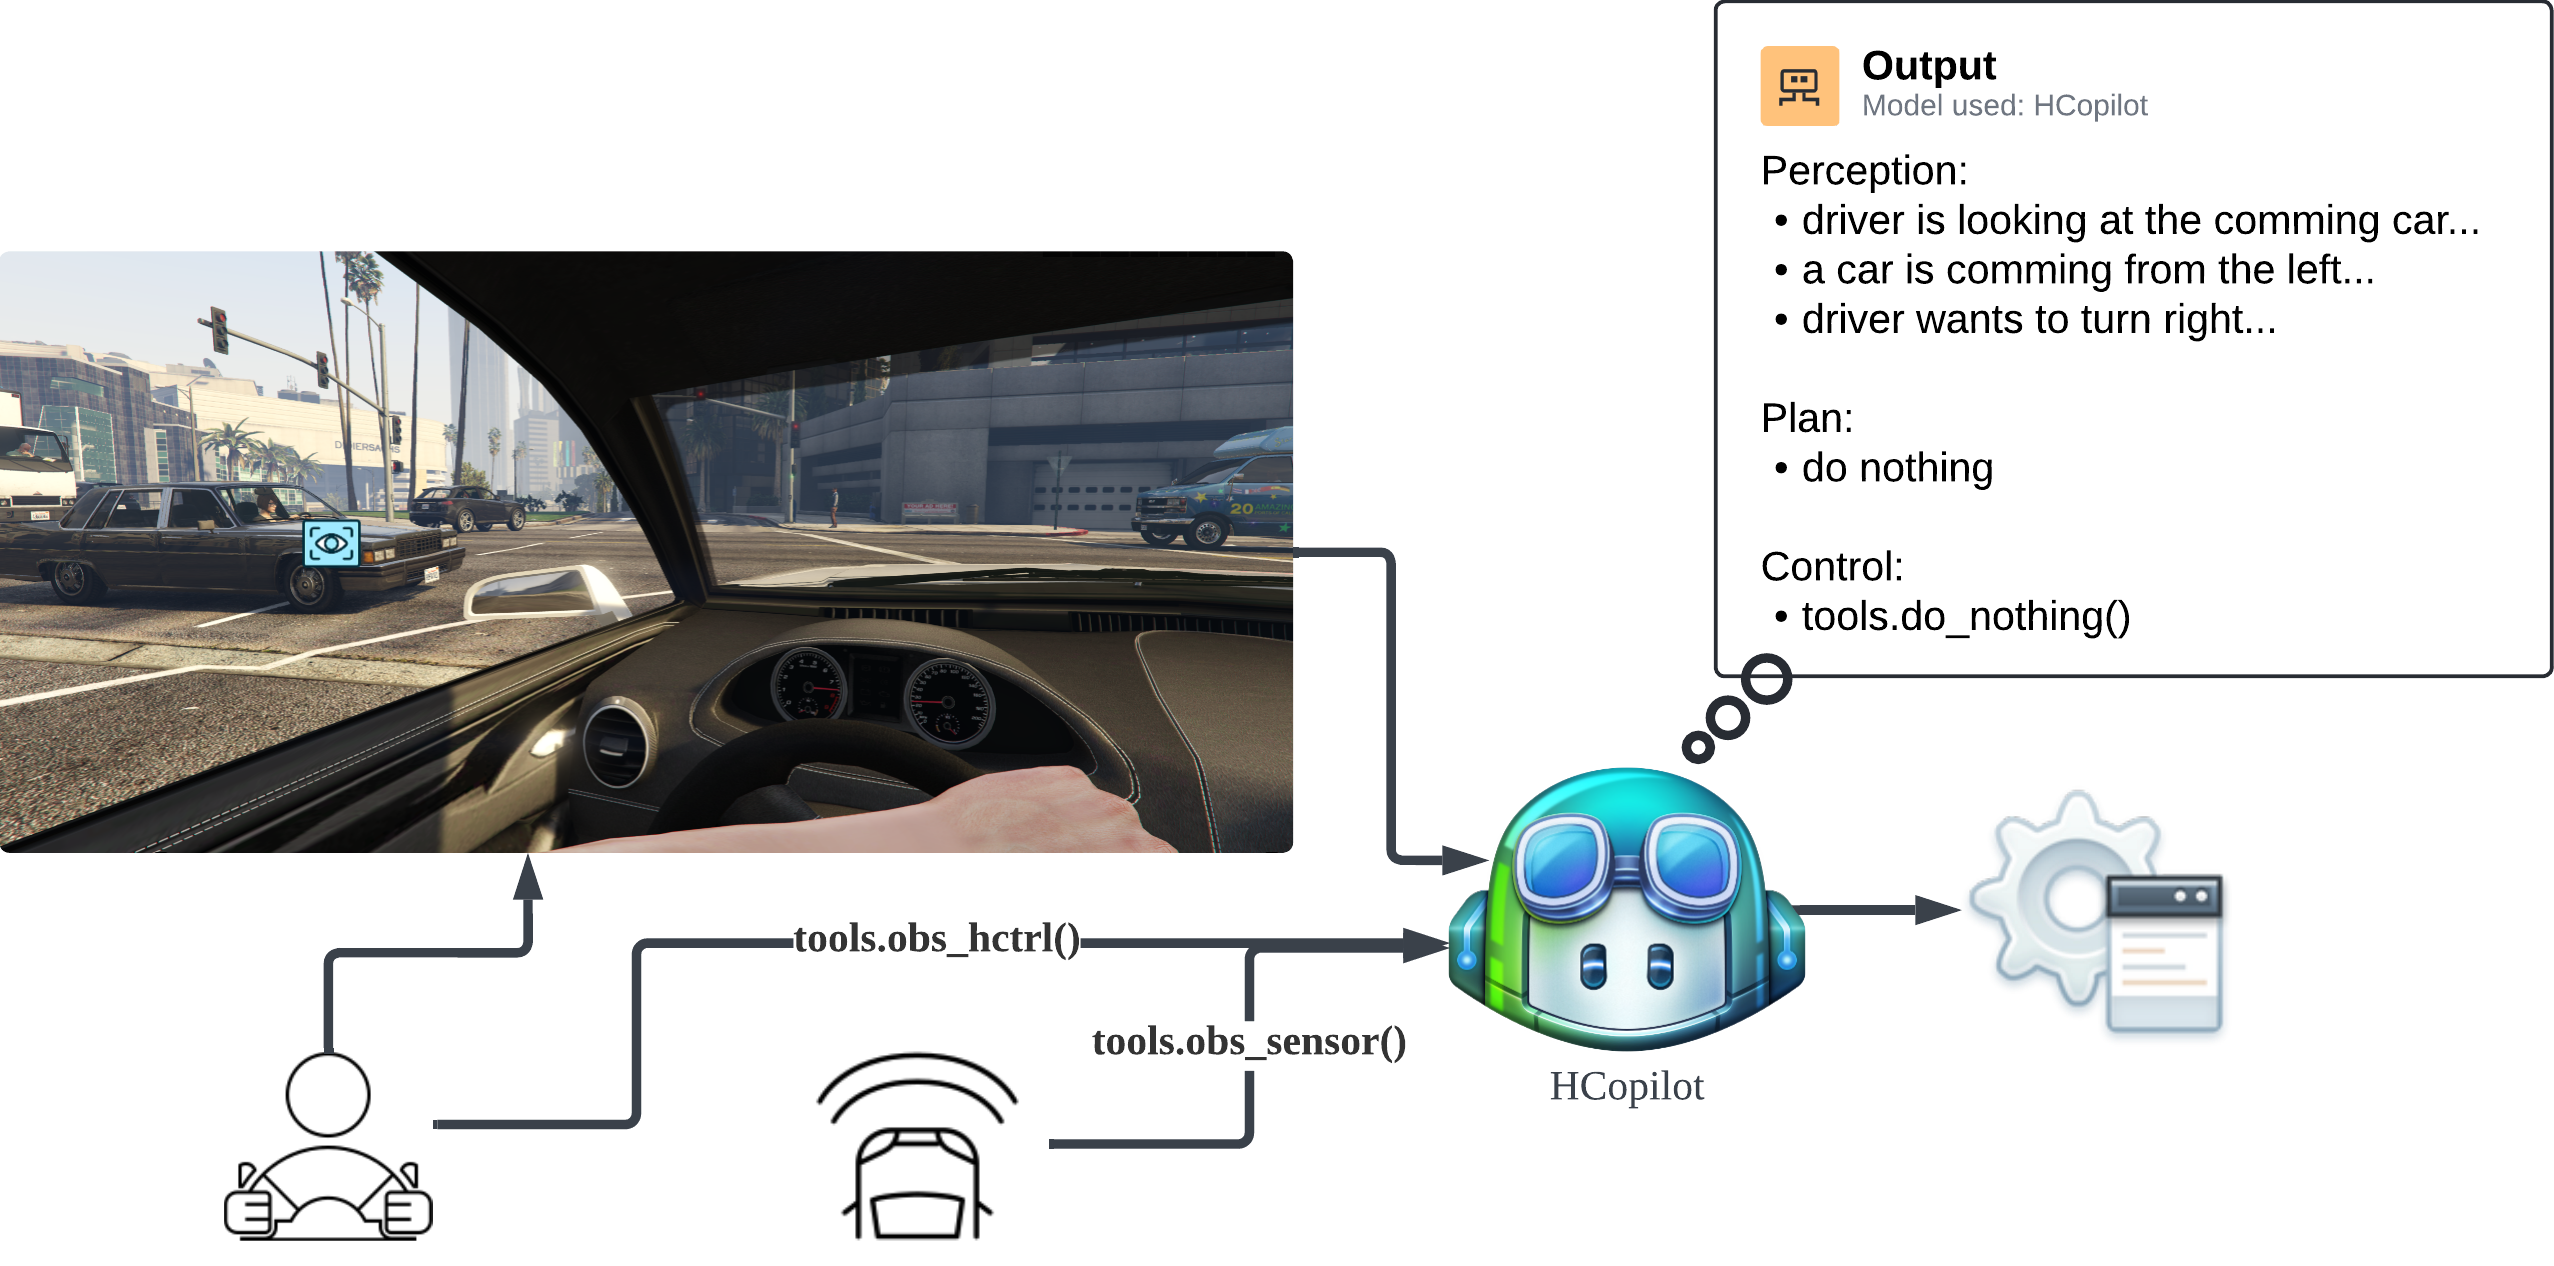
\includegraphics{C:/Users/Wiede/OneDrive - Queen Mary, University of London/Documentation/Projects/HCockpit/docs/figures/s-2-2.png}

\subsubsection{Scenario 3: Too Bright to
See}\label{scenario-3-too-bright-to-see}

In the scenario depicted in Figure x, the driver encounters direct
sunlight. A vehicle from the left approaches, unnoticed by the driver
due to glare, who opts to proceed slowly. HCopilot, noting this, chooses
to display a real-time video of vehicle v-100 on the HUD and issues a
voice alert, prioritizing the threat over enhancing spatial awareness.

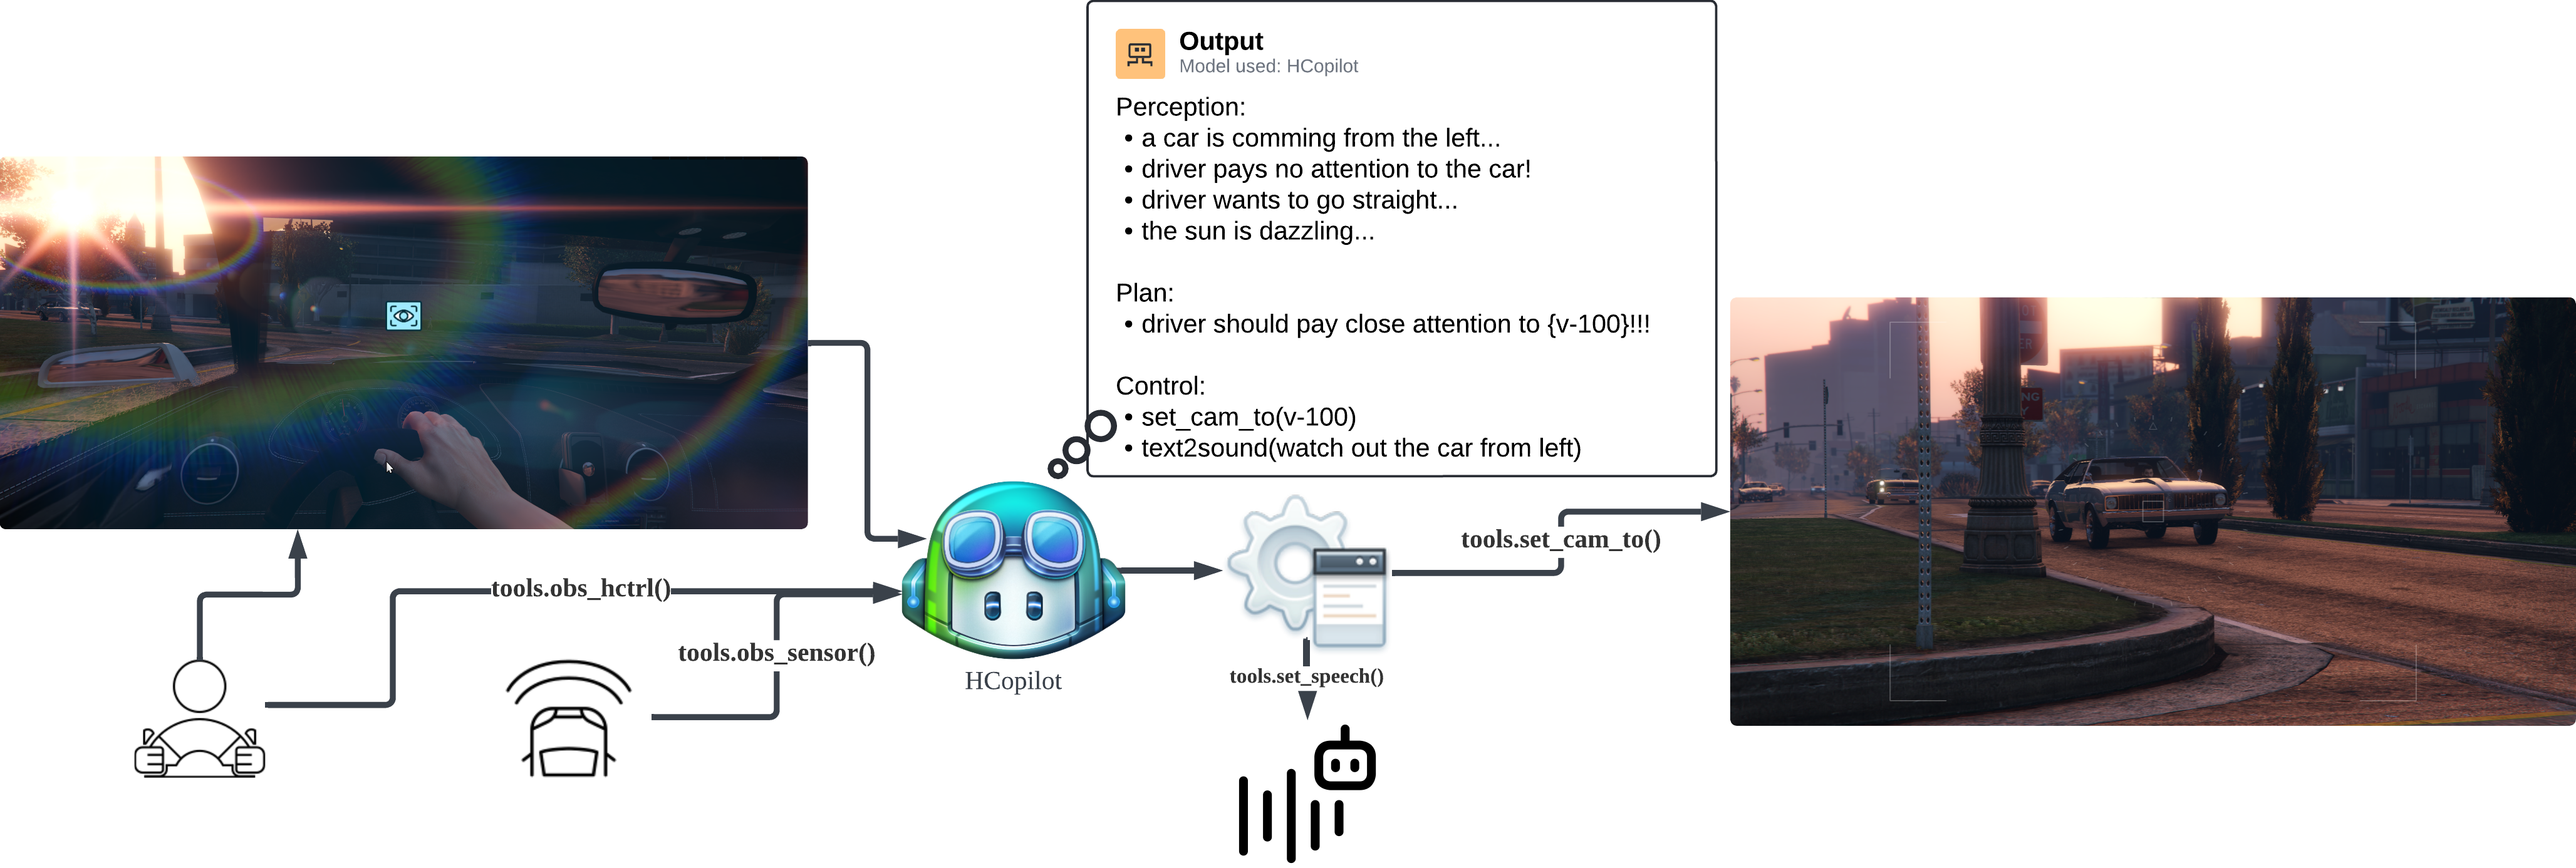
\includegraphics{C:/Users/Wiede/OneDrive - Queen Mary, University of London/Documentation/Projects/HCockpit/docs/figures/s-3.png}

\subsubsection{Scenario 4: Blind Area}\label{scenario-4-blind-area}

In the scenario shown in Figure x, the driver is checking a blind spot.
HCopilot opts to enhance situational awareness by displaying a real-time
video of the vehicle in the blind spot on the HUD, without using a voice
alert as the driver is already aware of the potential threat.

\includegraphics{C:/Users/Wiede/OneDrive - Queen Mary, University of London/Documentation/Projects/HCockpit/docs/figures/s-4.png}

\subsubsection{Scenario 5: Low
Attention}\label{scenario-5-low-attention}

In the scenario shown in Figure x, the driver is approaching an
intersection, focused on a mobile phone. HCopilot chooses to issue a
voice alert for the driver to prepare to brake, to avoid a collision
with the vehicle ahead.

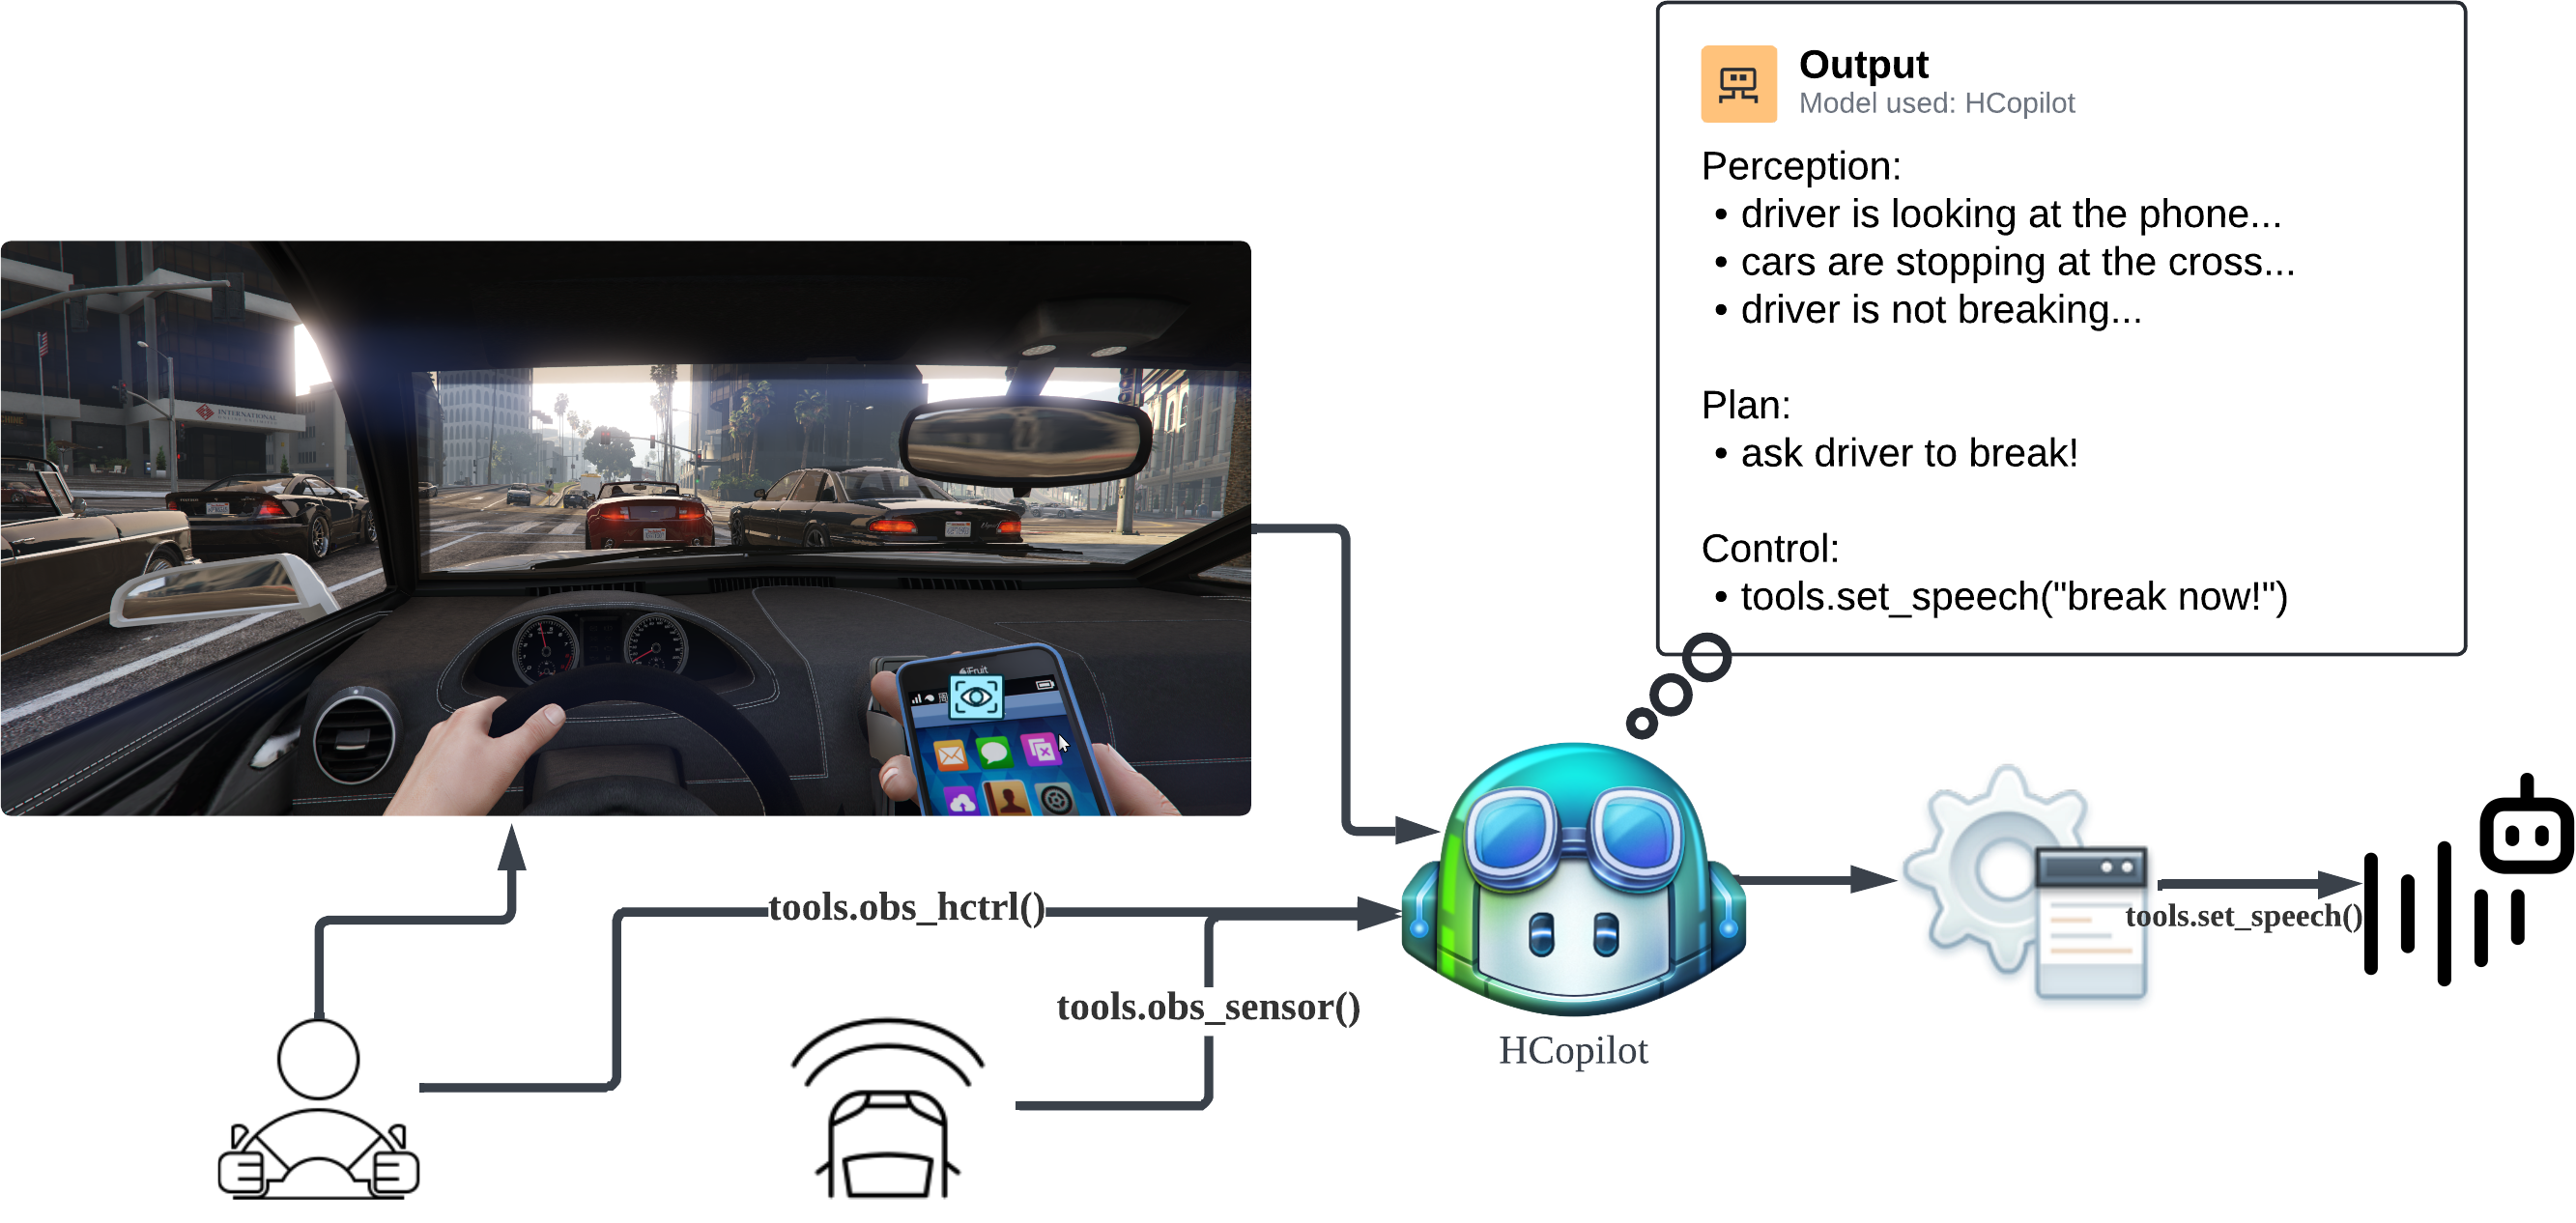
\includegraphics{C:/Users/Wiede/OneDrive - Queen Mary, University of London/Documentation/Projects/HCockpit/docs/figures/s-5.png}

\subsubsection{Discussion}\label{discussion}

HCopilot\textquotesingle s implementation showcases its effectiveness
and adaptability in complex urban driving environments. Through five
different driving scenarios, it is observed how HCopilot enhances the
driver\textquotesingle s situational awareness and safety through
real-time video streams and voice alerts. Specifically:

\begin{enumerate}
\def\labelenumi{\arabic{enumi}.}
\item
  \textbf{Effectiveness in Enhancing Situational Awareness}: In all
  scenarios, HCopilot effectively enhances environmental awareness by
  providing additional visual information and voice alerts, aiding
  drivers in making safer decisions, especially during lane changes,
  blind spot checks, and low attention scenarios.
\item
  \textbf{Adaptability and Intelligence of the System}: HCopilot
  demonstrates adaptability by adjusting its assistance strategy based
  on the driver\textquotesingle s behavior and changes in the external
  environment. For example, it ceases video streaming when it detects
  that the driver has noticed a potential threat, reducing information
  overload and showing an understanding of human behavior.
\item
  \textbf{Enhancement of Driving Experience}: While
  HCopilot\textquotesingle s interventions primarily enhance safety,
  they also improve the driving experience by reducing uncertainty and
  stress, making the driving process more relaxed and enjoyable.
  However, this positive impact needs validation across a broader
  driving population to ensure the system\textquotesingle s universal
  applicability and acceptance.
\end{enumerate}

\subsection{Conclusion and Future
Work}\label{conclusion-and-future-work}

\subsubsection{Conclusion}\label{conclusion}

This paper introduces a novel human-agent collaboration (HAC) framework
centered around large multimodal models (LMMs) to enhance situational
awareness (SA) in the cockpit. By integrating the perceptual and control
capabilities of human drivers and AI driving systems, the HCockpit
architecture successfully facilitates effective communication and
collaboration between humans and machines. The experimental results
demonstrate significant improvements in the driving experience and
safety, especially in scenarios involving blind spots and distracted
driving.

The technical implementation leverages the latest LMM, such as GPT-4
Turbo, allowing HCockpit to understand complex traffic environments and
human driver intentions, generating appropriate tasks and control
commands. Additionally, the designed communication mechanism ensures
transparency in system decisions, helping to enhance human understanding
and trust in the system.

Despite achievements, challenges such as precise alignment of multimodal
data and real-time data processing to meet system performance
requirements were encountered. Solutions to these issues largely rely on
continuous optimization of data processing techniques and algorithm
improvements.

Given more time for this project, exploration of advanced techniques for
multimodal data fusion to improve system accuracy and response times
would be pursued. Further, incorporating more user feedback mechanisms
to optimize the human-machine interaction interface would be considered.

\subsubsection{Reflection}\label{reflection}

This project was not only a technical challenge but also a profound
learning and growth experience. Through this research, a deeper
understanding of the potential and challenges of artificial intelligence
in practical applications was gained. Moreover, experiences in team
discussions taught effective communication and problem-solving under
pressure, significantly benefiting professional development.

The successful implementation of the project validates the research
direction and methodology, positively impacting academic and personal
development. It enhanced technical capabilities and improved project
management and decision-making skills.

\subsubsection{Future Work}\label{future-work}

Future research will continue in the following directions:

\begin{enumerate}
\def\labelenumi{\arabic{enumi}.}
\item
  \textbf{Entity Alignment Optimization}: Improving entity alignment
  techniques between different perspectives to enhance overall system
  performance and accuracy.
\item
  \textbf{Gaze Point Embedding Techniques}: Exploring embedding driver
  gaze data in vector form into the system decision-making process for
  more accurate behavior prediction and assistance.
\item
  \textbf{Local Real-Time Operation of LMMs}: Researching how to run
  large multimodal models in real-time locally, reducing reliance on
  cloud computing resources and enhancing system responsiveness and
  reliability.
\item
  \textbf{Unified and Standardized Cockpit Device Control Interface}:
  Collaborating with industry peers to promote the establishment of a
  unified and standardized cockpit device control interface, enabling
  seamless integration from high-level HAC tasks to specific device
  controls.
\end{enumerate}

Through these studies, further enhancement of HCockpit\textquotesingle s
performance and practicality, contributing to the development of future
intelligent transportation systems, is anticipated.

\subsection{References}\label{references}

\subsection{Acknowledgement}\label{acknowledgement}

\subsection{Appendices}\label{appendices}

\#\# Risk and Environmental Impact Assessment

\end{document}
